\chapter{Desarrollo realizado}

Como se ha comentado previamente, se ha intentado mantener la modularidad en todo el desarrollo asociado al proyecto. Esto, aunque no minimice el tamaño del código, tiene las siguientes ventajas:

\begin{itemize}
	\item{Reaprovechamiento de código para otras aplicaciones.}
	\item{Aislamiento de los errores: mayor facilidad para encontrarlos y menor extensión de estos.}
	\item{El paradigma empleado (Python es orientado a objetos) obliga a pensar de manera modular.}
\end{itemize}

En el momento actual están realizadas las siguientes aplicaciones

\section{Base de datos de accesos}
Se encuentra finalizada, pero todavía es susceptible a cambios. Se ha implementado sobre SQLite debido a la sencillez y a que el SQL empleado es bastante estándar (sería sencillo pasarla a otro sistema de gestión de bases de datos).

\section{Interfaz de Gestión de accesos}
La Interfaz de gestión de accesos será la interfaz sobre la cual se podrán :

\begin{itemize}
	\item{Consultar y modificar los datos de los empleados}
	\item{Consultar y modificar los accesos de estos}
\end{itemize}

Se ha considerado la siguiente interfaz para ver y/o modificar los datos de los empleados:
\begin{figure}[h!]
        \centering
        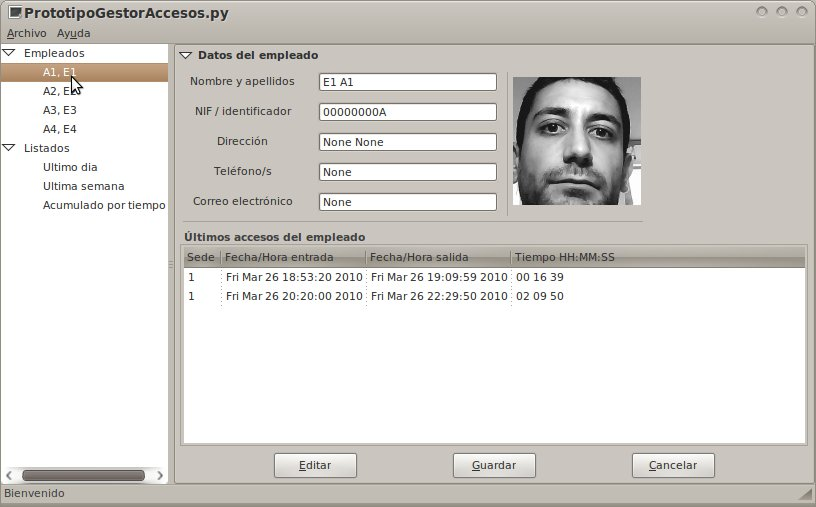
\includegraphics[width=14cm]{PrototipoGestorAccesosEmpleado.jpg}
        \caption{Gestión de accesos - Vista de empleado}
	\label{fig:gestion_accesos_emp}
\end{figure}

Y para ejecutar los listados se ha considerado que la siguiente interfaz tiene la información correcta
\begin{figure}[h!]
        \centering
        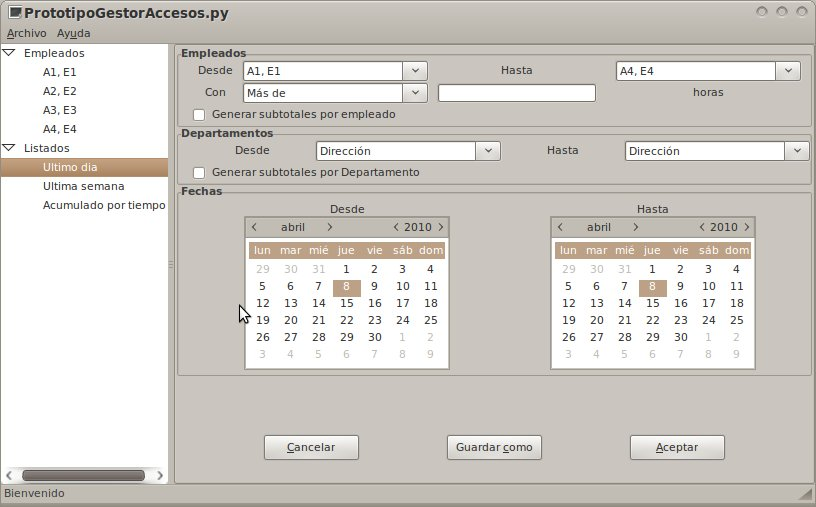
\includegraphics[width=14cm]{PrototipoGestorAccesosListados.jpg}
        \caption{Gestion de accesos - Vista de listado}
	\label{fig:gestion_accesos_list}
\end{figure}

En estos momentos está por finalizar. Falta la parte referente a listados, mejorar los temas de configuración y de tratamiento de errores, diálogos ``Acerca de'' y pulir detalles al respecto.

\section{Base de datos biométricos}
Es bastante sencilla: únicamente debe contener un identificador por cada individuo y una referencia a su signature. De momento no está implementada, pero se prevee bastante sencilla y no se descarta el unirla a la base de datos de accesos.

\section{Interfaz de Reconocimiento}
Esta aplicación debe instalarse en el punto de control de acceso.

\begin{itemize}
	\item{Requiere tener una webcam configurada.}
	\item{Es muy aconsejable que las condiciones de iluminación sean homogéneas.}
	\item{Consume bastante tiempo de procesador.}
\end{itemize}

La interfaz es relativamente sencilla, como se puede comprobar en la figura \ref{fig:reconocimiento}. Las opciones que tiene son sencillas: paso a escala de grises, encuadre de rasgos y/o de cara. 
\begin{figure}[h!]
        \centering
        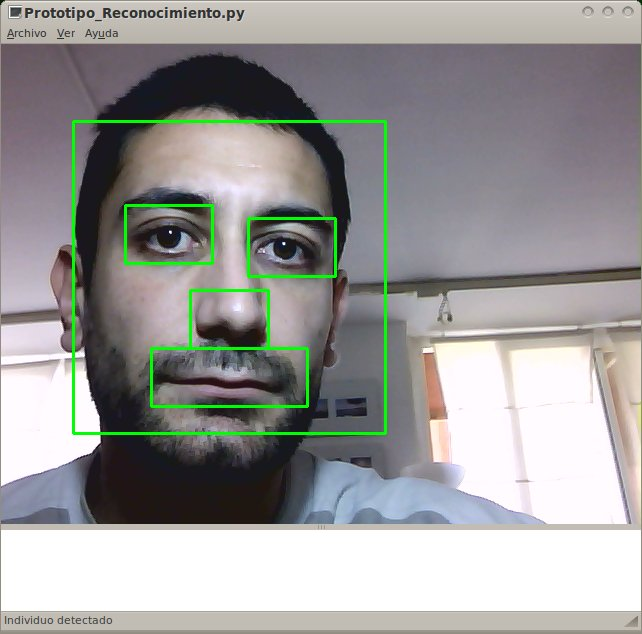
\includegraphics[width=14cm]{PrototipoReconocimiento.jpg}
        \caption{Interfaz de Reconocimiento (prototipo)}
	\label{fig:reconocimiento}
\end{figure}

Faltan por pulir detalles en cuanto a diálogos de configuración, tratamiento de excepciones y diálogo de "Acerca de". Comparte el diálogo de configuración (que se muestra en las figura \ref{fig:prefs_dialog}) con la Interfaz de captura.

\section{Interfaz de Captura}

Es muy similar a la Interfaz de reconocimiento, de hecho está ideada para ejecutarse en el mismo puesto que la de gestión de accesos. Difiere de esta en que solicita la introducción de un identificador para poder dar de alta a los individuos y bajo esto, se muestra la face signature capturada (escalada al tamaño de la ventana). Tiene los mismos requerimientos y aproximadamente el mismo consumo.

\begin{figure}[h!]
        \centering
        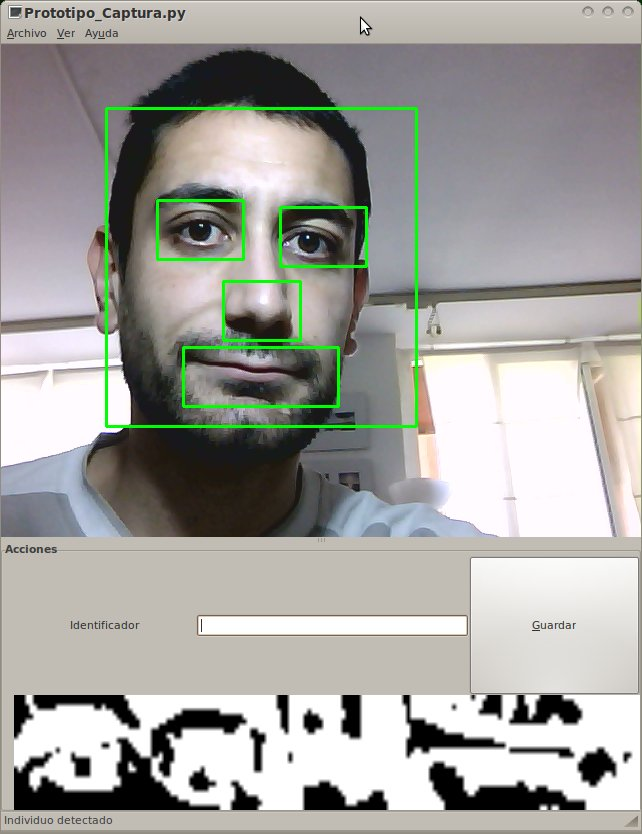
\includegraphics[width=14cm]{PrototipoCaptura.jpg}
        \caption{Interfaz de Captura (prototipo)}
	\label{fig:captura}
\end{figure}

En cuanto a la configuración de la webcam y de las bases de datos de acceso y biométricos, se configuran mediante el diálogo de preferencias (que es común a la interfaz de acceso y de captura), y que consta de las pestañas que se ven en las figura \ref{fig:prefs_dialog}.

\begin{figure}[h!]
        \centering
        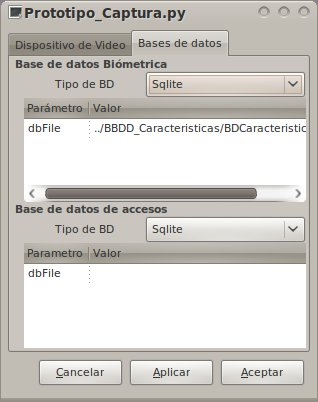
\includegraphics[width=6cm]{PreferencesDialogDB.jpg}
        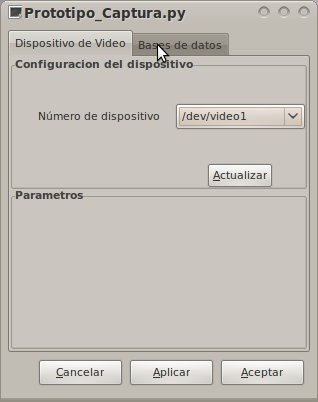
\includegraphics[width=6cm]{PreferencesDialogVideo.jpg}
        \caption{Diálogo de configuración (base de datos y vídeo)}
	\label{fig:prefs_dialog}
\end{figure}


De igual manera que las aplicaciones anteriores, tampoco está finalizada, faltándole los mismos puntos citados para éstas.
